\documentclass[10pt]{article}
\usepackage[T1]{fontenc}

% Document Details
\newcommand{\CLASS}{AMATH 585}
\newcommand{\assigmentnum}{Assignment 7}

\usepackage[margin = 1.15in, top = 1.25in, bottom = 1.in]{geometry}

\usepackage{titling}
\setlength{\droptitle}{-6em}   % This is your set screw
\date{}
\renewcommand{\maketitle}{
	\clearpage
	\begingroup  
	\centering
	\LARGE \sffamily\textbf{\CLASS} \Large \assigmentnum\\[.8em]
	\large Tyler Chen\\[1em]
	\endgroup
	\thispagestyle{empty}
}
 % Title Styling
\usepackage{tocloft}
\renewcommand{\cfttoctitlefont}{\Large\sffamily\bfseries}
\renewcommand{\cftsecfont}{\normalfont\sffamily\bfseries}
\renewcommand{\cftsubsecfont}{\normalfont\sffamily}
\renewcommand{\cftsubsubsecfont}{\normalfont\sffamily}

\makeatletter
\let\oldl@section\l@section
\def\l@section#1#2{\oldl@section{#1}{\sffamily\bfseries#2}}

\let\oldl@subsection\l@subsection
\def\l@subsection#1#2{\oldl@subsection{#1}{\sffamily#2}}

\let\oldl@subsubsection\l@subsubsection
\def\l@subsubsection#1#2{\oldl@subsubsection{#1}{\sffamily#2}}
 % General Styling


\usepackage{enumitem}

% Figures
\usepackage{subcaption}

% TikZ and Graphics
\usepackage{tikz, pgfplots}
\pgfplotsset{compat=1.12}
\usetikzlibrary{patterns,arrows}
\usepgfplotslibrary{fillbetween}

\usepackage{pdfpages}
\usepackage{adjustbox}

\usepackage{lscape}
\usepackage{titling}
\usepackage[]{hyperref}


% Header Styling
\usepackage{fancyhdr}
\pagestyle{fancy}
\lhead{\sffamily \CLASS}
\rhead{\sffamily Chen \textbf{\thepage}}
\cfoot{}

% Paragraph Styling
\setlength{\columnsep}{1cm}
\setlength{\parindent}{0pt}
\setlength{\parskip}{5pt}
\renewcommand{\baselinestretch}{1}

% TOC Styling
\usepackage{tocloft}
\iffalse
\renewcommand{\cftsecleader}{\cftdotfill{\cftdotsep}}

\renewcommand\cftchapafterpnum{\vskip6pt}
\renewcommand\cftsecafterpnum{\vskip10pt}
\renewcommand\cftsubsecafterpnum{\vskip6pt}

% Adjust sectional unit title fonts in ToC
\renewcommand{\cftchapfont}{\sffamily}
\renewcommand{\cftsecfont}{\bfseries\sffamily}
\renewcommand{\cftsecnumwidth}{2em}
\renewcommand{\cftsubsecfont}{\sffamily}
\renewcommand{\cfttoctitlefont}{\hfill\bfseries\sffamily\MakeUppercase}
\renewcommand{\cftaftertoctitle}{\hfill}

\renewcommand{\cftchappagefont}{\sffamily}
\renewcommand{\cftsecpagefont}{\bfseries\sffamily}
\renewcommand{\cftsubsecpagefont}{\sffamily}
\fi
 % General Styling
% Code Display Setup
\usepackage{listings,lstautogobble}
\usepackage{lipsum}
\usepackage{courier}
\usepackage{catchfilebetweentags}

\lstset{
	basicstyle=\small\ttfamily,
	breaklines=true, 
	frame = single,
	rangeprefix=,
	rangesuffix=,
	includerangemarker=false,
	autogobble = true
}


\usepackage{algorithmicx}
\usepackage{algpseudocode}

\newcommand{\To}{\textbf{to}~}
\newcommand{\DownTo}{\textbf{downto}~}
\renewcommand{\algorithmicdo}{\hspace{-.2em}\textbf{:}}
 % Code Display Setup
% AMS MATH Styling
\usepackage{amsmath, amssymb}
\newcommand{\qed}{\hfill\(\square\)}

%\newtheorem*{lemma}{Lemma} 
%\newtheorem*{theorem}{Theorem}
%\newtheorem*{definition}{Definition}
%\newtheorem*{prop}{Proposition}
%\renewenvironment{proof}{{\bfseries Proof.}}{}


% mathcal
\newcommand{\cA}{\ensuremath{\mathcal{A}}}
\newcommand{\cB}{\ensuremath{\mathcal{B}}}
\newcommand{\cC}{\ensuremath{\mathcal{C}}}
\newcommand{\cD}{\ensuremath{\mathcal{D}}}
\newcommand{\cE}{\ensuremath{\mathcal{E}}}
\newcommand{\cF}{\ensuremath{\mathcal{F}}}
\newcommand{\cG}{\ensuremath{\mathcal{G}}}
\newcommand{\cH}{\ensuremath{\mathcal{H}}}
\newcommand{\cI}{\ensuremath{\mathcal{I}}}
\newcommand{\cJ}{\ensuremath{\mathcal{J}}}
\newcommand{\cK}{\ensuremath{\mathcal{K}}}
\newcommand{\cL}{\ensuremath{\mathcal{L}}}
\newcommand{\cM}{\ensuremath{\mathcal{M}}}
\newcommand{\cN}{\ensuremath{\mathcal{N}}}
\newcommand{\cO}{\ensuremath{\mathcal{O}}}
\newcommand{\cP}{\ensuremath{\mathcal{P}}}
\newcommand{\cQ}{\ensuremath{\mathcal{Q}}}
\newcommand{\cR}{\ensuremath{\mathcal{R}}}
\newcommand{\cS}{\ensuremath{\mathcal{S}}}
\newcommand{\cT}{\ensuremath{\mathcal{T}}}
\newcommand{\cU}{\ensuremath{\mathcal{U}}}
\newcommand{\cV}{\ensuremath{\mathcal{V}}}
\newcommand{\cW}{\ensuremath{\mathcal{W}}}
\newcommand{\cX}{\ensuremath{\mathcal{X}}}
\newcommand{\cY}{\ensuremath{\mathcal{Y}}}
\newcommand{\cZ}{\ensuremath{\mathcal{Z}}}

% mathbb
\usepackage{bbm}
\newcommand{\bOne}{\ensuremath{\mathbbm{1}}}

\newcommand{\bA}{\ensuremath{\mathbb{A}}}
\newcommand{\bB}{\ensuremath{\mathbb{B}}}
\newcommand{\bC}{\ensuremath{\mathbb{C}}}
\newcommand{\bD}{\ensuremath{\mathbb{D}}}
\newcommand{\bE}{\ensuremath{\mathbb{E}}}
\newcommand{\bF}{\ensuremath{\mathbb{F}}}
\newcommand{\bG}{\ensuremath{\mathbb{G}}}
\newcommand{\bH}{\ensuremath{\mathbb{H}}}
\newcommand{\bI}{\ensuremath{\mathbb{I}}}
\newcommand{\bJ}{\ensuremath{\mathbb{J}}}
\newcommand{\bK}{\ensuremath{\mathbb{K}}}
\newcommand{\bL}{\ensuremath{\mathbb{L}}}
\newcommand{\bM}{\ensuremath{\mathbb{M}}}
\newcommand{\bN}{\ensuremath{\mathbb{N}}}
\newcommand{\bO}{\ensuremath{\mathbb{O}}}
\newcommand{\bP}{\ensuremath{\mathbb{P}}}
\newcommand{\bQ}{\ensuremath{\mathbb{Q}}}
\newcommand{\bR}{\ensuremath{\mathbb{R}}}
\newcommand{\bS}{\ensuremath{\mathbb{S}}}
\newcommand{\bT}{\ensuremath{\mathbb{T}}}
\newcommand{\bU}{\ensuremath{\mathbb{U}}}
\newcommand{\bV}{\ensuremath{\mathbb{V}}}
\newcommand{\bW}{\ensuremath{\mathbb{W}}}
\newcommand{\bX}{\ensuremath{\mathbb{X}}}
\newcommand{\bY}{\ensuremath{\mathbb{Y}}}
\newcommand{\bZ}{\ensuremath{\mathbb{Z}}}

% alternative mathbb
\newcommand{\NN}{\ensuremath{\mathbb{N}}}
\newcommand{\RR}{\ensuremath{\mathbb{R}}}
\newcommand{\CC}{\ensuremath{\mathbb{C}}}
\newcommand{\ZZ}{\ensuremath{\mathbb{Z}}}
\newcommand{\EE}{\ensuremath{\mathbb{E}}}
\newcommand{\PP}{\ensuremath{\mathbb{P}}}
\newcommand{\VV}{\ensuremath{\mathbb{V}}}
\newcommand{\cov}{\ensuremath{\text{Co}\VV}}
% Math Commands

\newcommand{\st}{~\big|~}
\newcommand{\stt}{\text{ st. }}
\newcommand{\ift}{\text{ if }}
\newcommand{\thent}{\text{ then }}
\newcommand{\owt}{\text{ otherwise }}

\newcommand{\norm}[1]{\left\lVert#1\right\rVert}
\newcommand{\snorm}[1]{\lVert#1\rVert}
\newcommand{\ip}[1]{\ensuremath{\left\langle #1 \right\rangle}}
\newcommand{\pp}[3][]{\frac{\partial^{#1}#2}{\partial #3^{#1}}}
\newcommand{\dd}[3][]{\frac{\d^{#1}#2}{\d #3^{#1}}}
\renewcommand{\d}{\ensuremath{\mathrm{d}}}

\newcommand{\indep}{\rotatebox[origin=c]{90}{$\models$}}




 % Math shortcuts
% Problem
\usepackage{floatrow}

\newenvironment{problem}[1][]
{\pagebreak
\noindent\rule{\textwidth}{1pt}\vspace{0.25em}
{\sffamily \textbf{#1}}
\par
}
{\par\vspace{-0.5em}\noindent\rule{\textwidth}{1pt}}

\newenvironment{solution}[1][]
{{\sffamily \textbf{#1}}
\par
}
{}

 % Problem Environment

\newcommand{\note}[1]{\textcolor{red}{\textbf{Note:} #1}}

\hypersetup{
   colorlinks=true,       % false: boxed links; true: colored links
   linkcolor=violet,          % color of internal links (change box color with linkbordercolor)
   citecolor=green,        % color of links to bibliography
   filecolor=magenta,      % color of file links
   urlcolor=cyan           % color of external links
}


\begin{document}
\maketitle


\begin{problem}[Problem 1]
The conjugate gradient method for solving a symmetric positive definite linear system
\( Ax=b \) can be written as below:
\vspace{.1in}

\begin{center}
\begin{tabular}{|l|} \hline
Given \( x_0 \), compute \( r_0 = b - A x_0 \), and set \( p_0 = r_0 \). \\
For \( k=1,2, \ldots \), \\
\( ~~ \) Compute \( A p_{k-1} \). \\
\( ~~ \) Set \( x_k = x_{k-1} + a_{k-1} p_{k-1} \), where $a_{k-1} = \frac{\langle r_{k-1} , r_{k-1} \rangle}
{\langle p_{k-1} , A p_{k-1} \rangle}$. \\
\( ~~ \) Compute \( r_k = r_{k-1} - a_{k-1} A p_{k-1} \). \\
\( ~~ \) Set \( p_k = r_k + b_{k-1} p_{k-1} \), where $b_{k-1} = \frac{\langle r_k , r_k \rangle}
{\langle r_{k-1} , r_{k-1} \rangle}$. \\
Endfor \\ \hline
\end{tabular}
\end{center}
\vspace{.1in}

\begin{enumerate}[label=(\alph*)]
\item
Show that the residual vectors \( r_0 , \ldots , r_k \) are orthogonal to each other (\( \langle r_i , r_j \rangle = 0 \) if \( i \neq j \)) and that the direction vectors  \( p_0 , \ldots , p_k \) are \( A \)-orthogonal (\( \langle p_i , A p_j \rangle = 0 \) if \( i \neq j \)).
[Hint:  First show that \( \langle r_1 , r_0 \rangle = \langle p_1 , A p_0 \rangle = 0 \) and then use induction on \( k \).]

\item
If \( A \) is the \( N \times N \) matrix of the 5-point operator for Poisson's equation on a square, count the number of operations (additions, subtractions, multiplications, and divisions) performed in each iteration.  (Show how you arrive at your result.)

\item
Compare your operation count in (b) to that of a Gauss-Seidel iteration applied to the same \( N \) by \( N \) 5-point matrix \( A \).  Also compare to the operation count for a multigrid V-cycle, using one Gauss-Seidel iteration on each visit to each grid level.
(Again, show how you derive your operation counts.)
\end{enumerate}
\end{problem}

\begin{solution}[Solution]

\begin{enumerate}[label=(\alph*)]
    \item 
        Note that \( p_0 = r_0 \) and \( A \) is SPD (implies self adjoint) so that \( \ip{x,Ay} = \ip{Ax,y} \). Then,
        \begin{align*}
            a_0 = \dfrac{\ip{r_0,r_0}}{\ip{ p_0, Ap_0 }} 
            = \dfrac{\ip{r_0,r_0}}{\ip{p_0,Ap_0}}
        \end{align*}
        

        We have,
        \begin{align*}
            \ip{r_1,r_0}  = \ip{ r_0-a_0Ap_0 , r_0 }
            = \ip{ r_0,r_0 } - \dfrac{\ip{r_0,r_0}}{\ip{p_0,Ap_0}} \ip{ A r_0, r_0} 
            = 0
        \end{align*}


        Likewise, using this result and the fact that \( b_0 = \ip{r_1,r_1}/\ip{r_0,r_0} \),
        \begin{align*}
            \ip{p_1,Ap_0} = \ip{r_1+b_0p_0,(r_0+r_1)/a_0}
            &= (\ip{r_1,r_0} + \ip{r_1,r_1} + b_0(\ip{r_0,r_0} + \ip{r_0,r_1}))/a_0
            = 0
        \end{align*}
        

        Suppose \( \ip{r_i,r_j} = \ip{p_i,A p_j } \) for all \( i,j \leq k \). 
        Then, for \( j < k \) we have,
        \begin{align*}
            \ip{A p_k,r_j} = \ip{A p_k, p_j - b_{j-1} p_{j-1}}
            = \ip{A p_k, p_j} - b_{j-1} \ip{A p_k, p_{j-1}}
            = 0
        \end{align*}
        
        Therefore, for \( j<k \) we have,
        \begin{align*}
            \ip{r_{k+1},r_j} = \ip{ r_k-a_kAp_k , r_j} = \ip{r_k,r_j} - a_k \ip{Ap_k,r_j} = 0
        \end{align*}
       
        If \( j = k \) then, \( a_k = \ip{r_k,r_k} / \ip{p_k,Ap_k} \) so,
        \begin{align*}
            \ip{r_{k+1},r_k} = \ip{r_k-a_kAp_k, r_k} = \ip{r_k,r_k} - a_k\ip{A p_k,p_k} = 0
        \end{align*}
        


        Using this fact, for \( j < k \), we now have,
        \begin{align*}
            \ip{r_{k+1},Ap_j} 
            = \ip{r_{k+1}, (r_j-r_{j+1})/a_j}
            = \ip{r_{k+1},r_j} / a_j - \ip{r_{k+1},r_{j+1}}/a_j
            = 0
        \end{align*}
        
        Therefore, for \( j < k \) we have,
        \begin{align*}
            \ip{p_{k+1}, A p_j} 
            = \ip{r_{k+1} + b_kp_k, A p_j}
            = \ip{r_{k+1}, Ap_j} + b_k \ip{p_k,Ap_j}
            = 0 
        \end{align*}

        If \( j = k \) then, since \( 1/a_k = \ip{p_k,Ap_k}/\ip{r_k,r_k} \) and \( b_k = \ip{r_{k+1},r_{k+1}}/\ip{r_k,r_k} \),
        \begin{align*}
            \ip{p_{k+1},A p_k} 
            &= \ip{r_{k+1}+b_kp_k,Ap_k}
            \\&= \ip{r_{k+1},(r_k-r_{k+1})/a_k} + b_k\ip{p_k,Ap_k}
            \\&= \ip{r_{k+1},r_k}/a_k - \ip{r_{k+1},r_{k+1}}/a_k + b_k\ip{p_k,Ap_k}
            = 0 
        \end{align*} 

        Given the base case proven earlier this proves \( \ip{r_i,r_j} = \ip{p_i, Ap_j} = 0 \) for all \( i\neq j \). \qed

    \item 
        Let \( A\in \RR^{n\times n} \). Then \( x_k, r_k, p_k \in \RR^n \). Computing a vector sum and scalar multiply each take \( n \) operations. Computing in inner product takes  \( 2n-1 \) floating point operations. If \( A \) is the matrix from the 5-point Poisson operator it has at most 5 entries in a given row. We assume that \( n \) is large so that the corners and edge cases do not matter. Therefore multiplying a single row of \( A \) by a vector will take 5 multiplications and 4 additions. We do this for all \( n \) rows. Therefore computing the product of \( A \) with a vector takes \( 9n \) operations.

The leading order term will be \( n \). We therefore do not count the divisions in the coefficients.

In the first line we have one matrix vector product.

In the second line we have two inner products, one vector add, and on scalar multiply.
However, one inner product was computed earlier, so we can skip this if we store it in memory.

In the third line one vector add, and on scalar multiply.

In the fourth line we have two inner product, one vector add, and one scalar multiply. 
However, again one inner product was computed earlier.

In total we have, one matrix vector product, two inner products, three vector additions, three scalar multiplies.
This gives,
\begin{align*}
    \Theta (9n + 2(2n) + 3(n) + 3(n)) = \Theta(19n) \text{ operations}
\end{align*}

    \item
        For a Gauss-Seidel step we first compute the residual \( b-Ax \) (one matrix vector product and one vector subtract).

        We then solve \( Me = r \). In GS iteration \( M \) is the lower triangular part of \( A \). Therefore there are at most 3 nonzero entries per row. Using back substitution, in each row we solve something like,
        \begin{align*}
            ax + by + cz = r && \Longleftrightarrow &&
            z = (r-ax-by)/c
        \end{align*}
        
        This is two multiplications, two subtractions and one division. Therefore for the whole matrix we have \( 5n \) operations.

        Finally, set \( x = x + e \) (one vector add).

        In total we have, one matrix vector product, one vector subtract, one sparse solve using back substitution, and one vector add. This gives,
        \begin{align*}
            \Theta(9n + n + 5n + n) = \Theta(16n) \text{ operations}
        \end{align*}
        
        \vspace{1em}


        Suppose we have a multi-grid V-cycle. At each level we do a Gauss-Seidel step, project, (do the iterative part), interpolate back, and do another Gauss-Seidel step.
        We assume a linear interpolation matrix, and the natural projection matrix.

        We will come up with an upper bound for the leading coefficient of the number of operations.

        We showed a Gauss-Seidel step takes \( \Theta(16n) \) operations.

        Our interpolation matrix averages either 1 point (if the point is in the coarse grid), 2 points (if it is between two points in the coarse gird), or 4 points (if the point is between 4 points in the coarse grid). In the worse case we average 4 points together (3 additions one division). This occurs for \( \mathcal{O} (n/4) \) points.

        Projecting down takes constant time since we do not do any floating point operations (although we do read and write to memory \( \mathcal{O} (n) \) times.

        Interpolating takes less than 9 multiplications and 8 additions for each of the \( (n-1)/2 \) rows.

        At one level we then have,
        \begin{align*}
            \Theta( 16n + 4(n/4) + 0 + 16n ) = \Theta( 33n ) \text{ operations}
        \end{align*}

        Suppose we make \( k \) steps until we can solve the final system easily (in \( \mathcal{O} (1) \). At each successive grid level the size of the matrices decreases by a factor of two for each dimension for a total factor of 4. Then the algorithm takes,
        \begin{align*}
            \sum_{k=0}^{n} \left( \dfrac{1}{4} \right)^k \Theta(33 n) \text{ operations}
        \end{align*}
        
        In the limit \( k\to \infty \) we have,
        \begin{align*}
            (4/3) \Theta(33 n) = \Theta(44n) \text{ operations}
        \end{align*}
        
        

        We note that reading and writing to the memory takes non-negligible time, especially for sparse array computations. Some things like scalar multiplications might not need to be computed at each stage either depending on the algorithm. In short, these computations are a good approximation to the actual result, but floating point operations are not the single most important thing, especially for large systems on large computers.

\end{enumerate}

\end{solution}

\begin{problem}[Problem 2]
Implement a 2-grid method for solving the 1D model problem with homogeneous Dirichlet boundary conditions:
\[
u_{xx} = f(x) ,~~u(0) = u(1) = 0.
\]
Use linear interpolation to go from the coarse grid with spacing \( 2h \) to the fine grid with spacing \( h \).  Take the projection matrix \( I_h^{2h} \), going from the fine grid to the coarse grid, to be \( 0.5 \) times the transpose of the interpolation matrix: \( I_h^{2h} = \frac{1}{2} ( I_{2h}^h )^T \). Use a multigrid V-cycle with 1 smoothing step on each visit to each grid level. Try weighted Jacobi and Gauss-Seidel as the smoothing step. Try several different values of the mesh spacing \( h \) and show that you achieve convergence to a fixed tolerance in a number of cycles that is independent of the mesh size.
\end{problem}

\begin{solution}[Solution]

We implement a general arbitrary depth V-cycle multigrid solver.
\lstinputlisting[linerange=\#<startMG>-\#<endMG>]{hw7_2.py}


We the solver with \( J=1 \) so that there are two grid levels. A sample solution is shown in Figure~\ref{sol} after the residual has reached a tolerance of \( 1^{-10} \).
\begin{figure}[H]\centering
    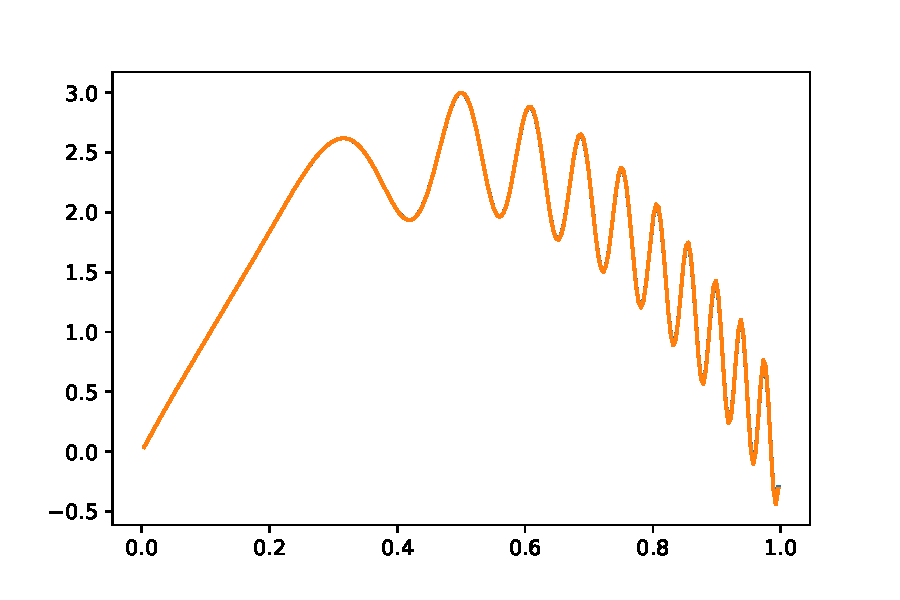
\includegraphics[width=0.48\textwidth]{img/mg_2_sol.pdf}
    \caption{Sample solution (orange) vs. actual solution (blue)}
\label{sol}
\end{figure}

We use a direct solve on the coarse grid, and one simple iteration smooth on the fine grid. Figure~\ref{mg} shows the number of iterations required for the residual to reach a tolerance of \( 1^{-10} \) using weighted Jacobi and Gauss-Seidel in the smoothing step. Note that the number of iterations does not change appreciably as the mesh size increases. 
\begin{figure}[H]\centering
    \begin{subfigure}{.48\textwidth}
        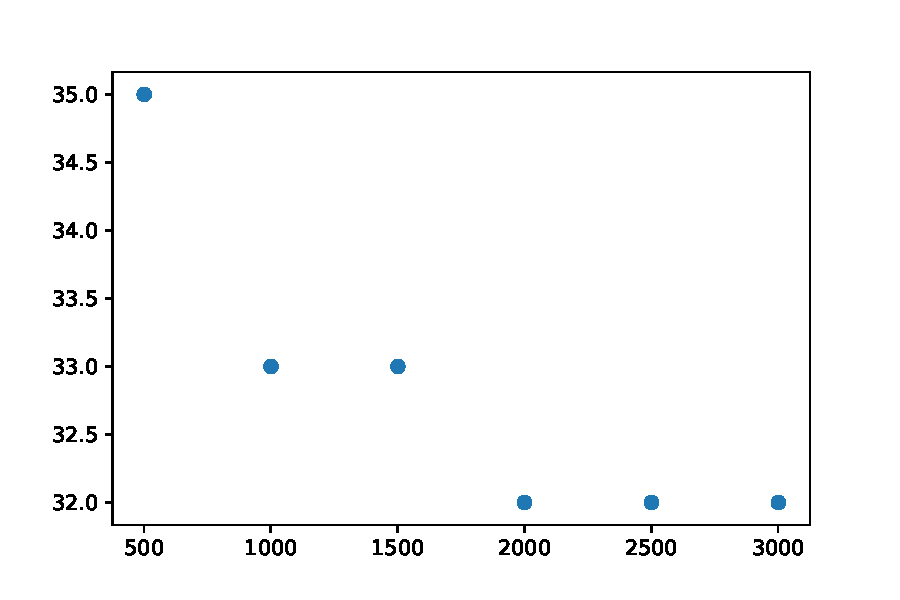
\includegraphics[width=\textwidth]{img/multigrid_j_1.pdf}
        \caption{weighted Jacobi ( \( \omega = 2/3 \))}
    \end{subfigure}
    \begin{subfigure}{.48\textwidth}
        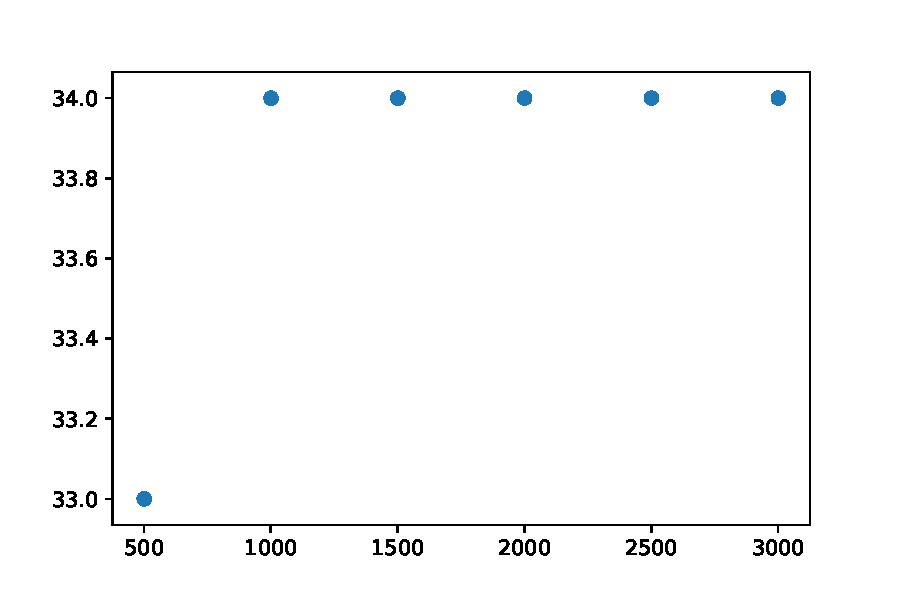
\includegraphics[width=\textwidth]{img/multigrid_gs_1.pdf}
        \caption{Gauss-Seidel}
    \end{subfigure}
    \caption{Number of iterations for residual to reach \( 1^{-10} \)}
\label{mg}
\end{figure}

\end{solution}

\begin{problem}[Problem 3]
\begin{enumerate}[label=(\alph*)]
\item
Consider an iteration of the form 
\[
x_k = x_{k-1} + M^{-1} ( b - A x_{k-1} ) ,
\]
for solving a nonsingular linear system \( Ax=b \).  Note that the error \( e_k := A^{-1} b - x_k \)
satisfies
\[
e_k = (I - M^{-1} A) e_{k-1} = \ldots = (I - M^{-1} A)^k e_0.
\]
Assume that \( \| e_0 \|_2 = 1 \) and that \( \| I - M^{-1} A \|_2 = \frac{1}{2} \). Estimate the number of iterations required to reduce the 2-norm of the error below \( 2^{-20} \). Show how you obtain your estimate.  Now suppose you know only that the spectral radius \( \rho ( I - M^{-1} A ) = \frac{1}{2} \).  Can you give an estimate of the number of iterations required to reduce the 2-norm of the error below \( 2^{-20} \)?  Explain why or why not.

    
\item Consider the GMRES algorithm applied to an \( n \) by \( n \) matrix \( A \) with the sparsity pattern pictured below:
\[
\left[ \begin{array}{ccccc}
\ast & \ast & \cdots & \ast & \ast \\
\ast & \ast & \cdots & \ast & 0 \\
0    & \ast & \cdots & \ast & 0 \\
\vdots  & \ddots & \ddots & \vdots & \vdots \\
0    & \cdots    & \cdots & \ast & 0 \end{array} \right] ,
\]
where the \( \ast \)'s represent nonzero entries.  Show that if the initial residual is the 
\( n \)th unit vector \( ( 0, \ldots , 0 , 1 )^T \), then the algorithm makes no progress until step \( n \).  Show that a matrix with this sparsity pattern can have {\em any} eigenvalues.  Conclude that eigenvalue information alone cannot be enough to ensure fast convergence of the GMRES algorithm.
\end{enumerate}
\end{problem}

\begin{solution}[Solution]

\begin{enumerate}
    \item
        Recall \( \norm{Ax}_2 \leq \norm{A}_2\norm{x}_2 \).

        We therefore have,
        \begin{align*}
            \norm{e_k}_2 = \norm{(I-M^{-1}A)^k e_0}
            \leq \norm{I-M^{-1}A}^k \norm{e_0}
            = 2^{-k}
        \end{align*}
        
        Therefore we have \( \norm{e_k} < 2^{-20} \) when \( k > 20 \).

        This is an upper bound, so depending on \( M \) and \( A \) the bound could be improved.

        We have \( \rho(A) \leq \norm{A}_2 \). However there is no relation in the other direction for general matrices \( A \). 

        Without knowing the structure of \( M \) we cannot bound the number of iterations required to reach some tolerance.

        If we knew \( M \) we might be able to find a bound which does not depend on \( A \) for some set of reasonable \( A \) (although this is not true for all \( A \) for the same reasons as above).

        Otherwise, if we know \( I-M^{-1}A \) is symmetric, then \( \rho(I-M^{-1}A) = \norm{I-M^{-1}A}_2 \) so we can use the above estimate.

    \item
        Observe that \( Ar_0 = (a_{1,n}, 0,\ldots, 0)^T \). Therefore \( A^2 r_0 \) has sparsity pattern \( (*,*,0\ldots,0)^T \) and \( A^3r_0 \) has sparsity pattern \( (*,*,*,0,\ldots, 0)^T \). Therefore, \( r_0 \) is orthogonal to \( A^k r_0 \) for \( k=1,\ldots, n-1 \).

        
        
        At step \( k \) the residual has the form,
        \begin{align*}
            r_k = r_0 - AQ_ky_k
        \end{align*}
        
        Recall the columns of \( Q_k \) form a basis for \( \mathcal{K}_k \). Therefore,
        \begin{align*}
            AQ_ky_k \in \operatorname{span}\{Ar_0, A^2r_0, \ldots, A^k r_0\} 
        \end{align*}
        
        Since \( AQ_ky_k \in \operatorname{span}\{Ar_0, A^2r_0, \ldots, A^k r_0\} \), then for any \( k<n \) we know \( r_k \) has a one in the last slot. Therefore \( \norm{r_k}_2 \geq 1 \). However since \( AQ_k \) is not full rank for \( k<n \), clearly there is some \( y_k \) such that \( AQ_ky_k = 0 \) so that \( \norm{r_k}_2 = 1 \). 

        Since the algorithm minimizes the residual it will pick \( y_k \in \operatorname{ker} AQ_k \) at each of these steps.

        This means the algorithm makes no progress for the first \( n-1 \) steps. However, at step \( n \) the algorithm is able to make progress.

        \vspace{1em}
        
        
        Let \( \{\lambda_k\}_{k=1}^{n} \) be any \( n \) complex numbers. Then there is a polynomial \( p(x) = c_0 + c_1x + \ldots + c_{n-1}x^{n-1} + t^n \) over \( \CC \) with each \( \overline{\lambda}_k \) as a root. 

        Let \( C \) be the companion matrix of \( p(x) \). Then each \( \overline{\lambda}_k \) is an eigenvalue of \( C \).

        Let \( Q \) be the matrix with ones on the antidiagonal. Then \( Q \) is unitary so that \( Q^*Q = I \).

        Explicitly we have,
        \begin{align*}
            C = 
            \left[\begin{array}{rrrrr}
                0 & 0 &\cdots & 0 & -c_0 \\
                1 & 0 & \cdots & 0 & -c_1 \\
                0 & 1 & \cdots & 0 & -c_2 \\
                \vdots & \vdots & \ddots  & \vdots & \vdots \\
                0 & 0 & \cdots & 1 & -c_{n-1}
            \end{array}\right]
            &&
            Q = 
            \left[\begin{array}{rrrrr}
                &&&&1\\
                &&&1\\
                &&\ddots\\
                &1\\
                1
            \end{array}\right]
        \end{align*}

        Observe,
        \begin{align*}
            (QCQ^*)^* = 
            \left[\begin{array}{rrrrr}
                -c_{n-1} & \cdots & -c_2 & -c_1 & -c_0 \\
                1 & \cdots & 0 & 0 & 0 \\
                \vdots & \ddots & \vdots & \vdots & \vdots \\
                0 & \cdots & 1 & 0 & 0\\
                0  & \cdots & 0 & 1 & 0\\
            \end{array}\right]
        \end{align*}
        
        Note that \( QCQ^* \) is a similarity transform of \( C \) and therefore the eigenvalues of \( QCQ^* \) are the \( \lambda_k \). The eigenvalues of the Hermetian conjugate of a matrix are the complex conjugate of the eigenvalues of the original matrix. This proves \( \lambda_k \) is an eigenvalue of \( (Q^*CQ)^* \) for \( k=1,2,\ldots, n \).

        Clearly this matrix has the desired form (in fact even stricter). Therefore, a (real) matrix with this sparsity pattern can have any (real or complex) eigenvalue.

        \vspace{1em}

        Together these two results mean that given any eigenvalues there is some matrix with these eigenvalues for with which GMRES does not make progress on until the \( n \)-th step.

\end{enumerate}
\end{solution}

\end{document}
